\chapter{Distributed File System}

\begin{multicols*}{2}
\noindent Distributed file system supports file accesses throughout an intranet. Requirements:
\begin{itemize}
    \item Access transparency: clients should use the same interface for accesses to local and remote files
    \item Location transparency: client should see a uniform file name space
    \item File replication to improve performance and enhance fault tolerance
    \item Consistency maintenance of replications
\end{itemize}

\section{Stateless versus Stateful Servers}

\noindent Stateful server remembers client’s previous operations, so the requests are inter-dependent. It has heavier demand on server and harder to set up or restore on crashes.\\

\noindent Stateless server does not remember client’s previous operations, so the request is independent of other requests. It is easier to set up and restore, less burden on server, but heavier demand on network\\

\noindent Stateless services are preferred for distributed file systems

\section{Sun Network File System}

\begin{center}
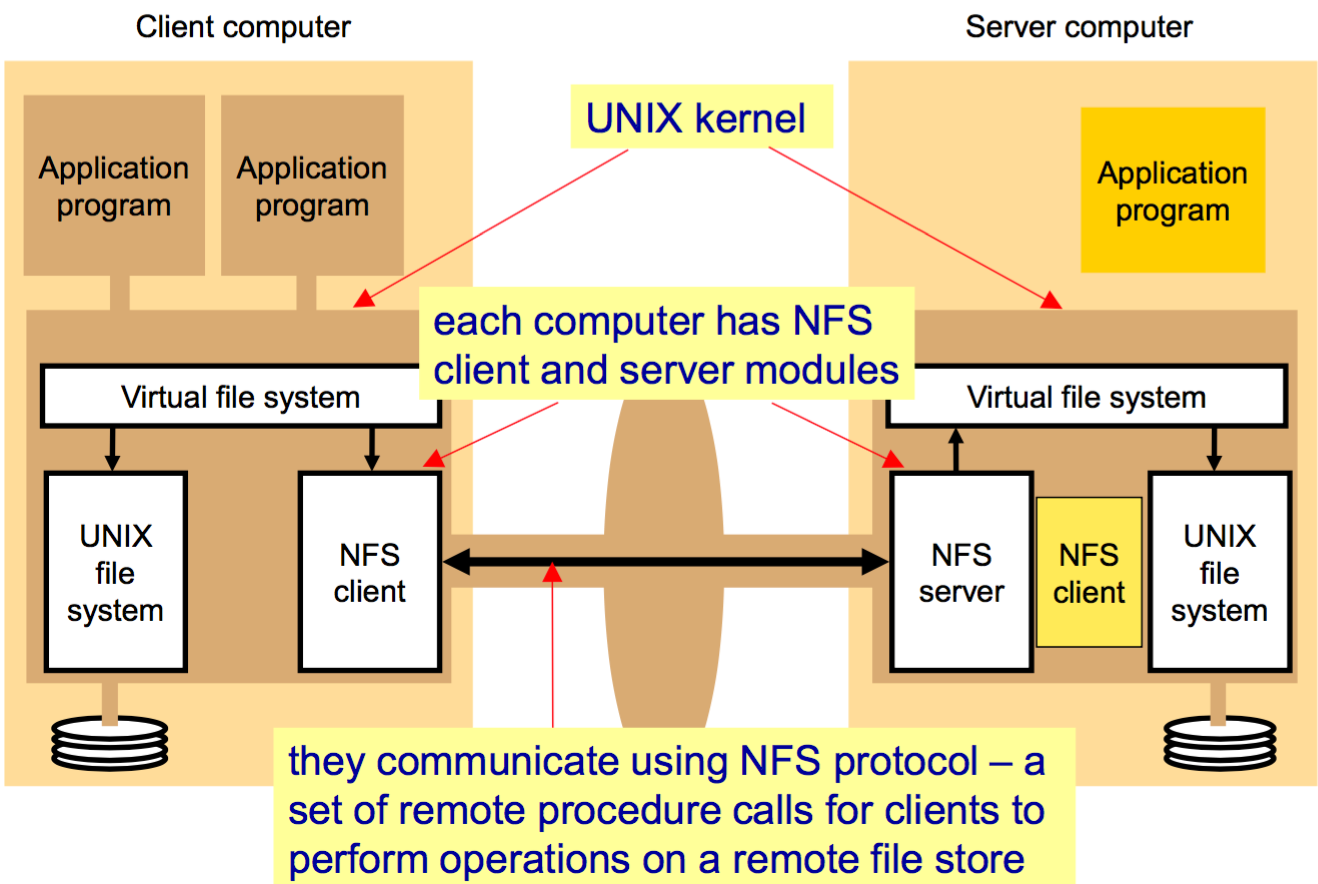
\includegraphics[width=8cm]{sun-file-system}
\end{center}

\noindent Each computer can act as both a client and a server.

\noindent File are accessed by file identifiers. File identifier is independent of the file name, created by the server hosting the file system and unique with respect to all files in the system. 

\subsection{Client-Server Communication}

\noindent NFS server operations are stateless and idempotent, so at-least-once invocation semantics can be used.\\

\noindent NFS client operations need to supply an interface suitable for use by conventional application programs. The interface emulates UNIX file system semantics. \\

\subsection{Mount Service}

\noindent File systems have to be exported by the server and be mounted by a client before they can be accessed by the client.\\

\noindent At the server, a mount service process runs at user level on each server. A file \verb|/etc/exports| contains the names of local file systems available for remote mounting and access list. \\

\noindent Client side use a modified UNIX mount command to request mounting, specifying remote host name, pathname of a directory in remote file system, and local name to be mounted. The command communicates with mount service process using PRC protocol. A table of mounted file systems is maintained at the client.\\

\noindent NFS does not enforce a single network-wide file name space. Clients can assign different local names to the same remote directory.\\

\noindent Pathnames are parsed, and their translation is performed in an iterative manner by clients. For example, if the root directory of a remote server is mounted, access to \verb|/bin/draw/readme| on the server requires three lookup request:
\begin{itemize}
    \item \verb|lookup(rootfh, "bin")| $\rightarrow$ \verb|bin| file handler
    \item \verb|lookup(binfh, "draw")| $\rightarrow$ \verb|draw| file handler
    \item \verb|lookup(drawfh, "readme")| $\rightarrow$ \verb|readme| file handler
\end{itemize}

\noindent To improve efficiency, we using caching to take advantage of reference locality. For example, if \verb|/bin/draw/install| is accessed soon after \verb|/bin/draw/readme| on the same server, only one lookup request to the server is needed.

\subsection{Client Caching}

\noindent NFS client caches file data at block level to reduce communication with server. However, writing operation by a client do not result in immediate updating of cached copies of the same file in other clients. To maintain cache consistency, clients are responsible for polling the server to check the currency of cached data they hold. \\

\noindent NFS provides a close approximation to one-copy semantics:
\begin{itemize}
    \item Each cache entry is tagged with two timestamps:
    \begin{enumerate}
        \item The last validation time of cache, $T_c$
        \item The last modified time of cached file at server $T_{\text{mclient}}$
    \end{enumerate}
    \item Entry is considered valid when $T-T_c < t$, where $t$ is a freshness interval and $T$ is currect time
    \item When client want to access a cached file:
    \begin{itemize}
        \item If $T-T_c<t$, read data from cache
        \item If $T-T_c\ge t$, get $T_{\text{mserver}}$ from server. If $T_{\text{mclient}}=T_{\text{mserver}}$, update $T_c$ and $T_{\text{mclient}}$ to current time. If $T_{\text{mclient}}<T_{\text{mserver}}$, send a new request to server to get new file.
    \end{itemize}
\end{itemize}

\subsection{Summary}

\noindent NFS achieves access transparency because application use the same file operations for both local and remote files.\\

\noindent NFS does not achieve location transparency because different clients can mount the same server directory to different local directories. 

\section{Andrew File System}

\noindent Andrew File System (AFS) are designed for scalability. AFS nodes are paritioned into two groups: (1) dedicated file servers and (2) a large number of clients. \\

\noindent Similar to NFS: 
\begin{itemize}
    \item Client can access to AFS files via normal UNIX file system operations.
    \item Venus clients and vice servers communicate using RPC
    \item Venus translates the pathnames into file identifiers using a step-by-step lookup
    \item File are accessed by file identifiers
\end{itemize}

\noindent Vice servers maintain a globally shared file name space. Clients have access to shared name space by means of a special local subdirectory \verb|/afs|. \\

\noindent Shared files are grouped into volumes for ease of replication.

\subsection{Server-side Replication}

\noindent Each file is contained in exactly one logical volumne and each logical volume may have several physical volumes. \\

\noindent Each logical volume is associated with a Replicated Volume Identifier (RVID, location and replication-independent) and each physical volume is associated with a Volume Identifier (VID, location-independent).\\

\noindent Each shared file is identified by a unique file identifier (RVID + file handle). \\

\noindent Consistency for AFS server-side replication is read-one, write-all. 

\subsection{Whole-file Serving and Caching}

\noindent Whole-file serving: entire files are transmitted to clients by AFS servers.\\

\noindent Whole-file caching: files transferred to a client are stored in a cache on local disk to satisfy future requests. When client close a file, the client transmits the updates to the server and retains the local copy.\\

\noindent AFS uses session update semantics to be more scalable. All other clients are able to see a modified file only after the file is closed by the client that modified it.\\

\noindent Callback mechanism is used to maintain cache consistency of client side. Vice server will issue a callback promise in \textit{valid} state to Venus client when the server sends a fresh file copy to client. When there is a update of the file at server side, the server will inform all clients with valid callback promise and remove these clients from its callback list. When a client receives a callback from the server, the client sets the callback promise to \textit{cancelled}.\\

\noindent However, if there is an update at server side before a client close a session / file, the callback has no effect on the file at currect session. If multiple clients write to a file concurrently, all update are silently lost except those of the last client closing the file. 

\subsection{Coda File System}

\noindent The main design goal of Coda file system is high availability. It allows clients to continue operation despite being disconnected from a server. Clients can use its locally cached copy of the files when disconnected from servers and reconcile later when the connection is established again. \\

\noindent To ensure client caches contain files that will be accessed during disconnection, we use hoarding technique, which fills the cache in advance with useful files:
\begin{itemize}
    \item We first ask user to specify useful files in a hoard database. Then, priorities for each file are computed using hoard database and information on recent file accesses.
    \item We fetch files in priority to reach equilibrium, when all cached files have higher priorities than uncached files, cache is full, all uncached files have zero priority, or cached files are up-to-date. 
    \item We do a hoard walk to periodically reorganize the cache to maintain equilibrium. 
\end{itemize}

\noindent There are 3 states of Coda client with respect to a volume: hoarding, emulation, and reintegration. 

\begin{center}
\begin{tikzpicture}[
node distance=1.5cm,
roundnode/.style={rectangle, draw=black, thin},
]
%Nodes
\node[roundnode](Hoarding){Hoarding};
\node[below=of Hoarding](dummy){};

\node[roundnode](Emulation)[left=of dummy]{Emulation};

\node[roundnode](Reintegration)[right=of dummy]{Reintegration};

\path[pil] (Reintegration) edge [bend right=45] node [pos=0.5, sloped, above, align=center] {Reintegration\\Completed} (Hoarding);
\path[pil] (Hoarding) edge [bend right=45] node [pos=0.5, sloped, above] {Disconnection} (Emulation);
\path[pil] (Emulation) edge [bend right=20] node [pos=0.5, sloped, below] {Reconnection} (Reintegration);
\path[pil] (Reintegration) edge [bend right=20] node [pos=0.5, sloped, above] {Disconnection} (Emulation);

\end{tikzpicture}
\end{center}

\noindent When the connection is established again, updates made to files during disconnection are transferred to the server. In case of conflicts, we can use automatic conflict resolution or manual intervention to resolve conflict. However, conflicts are rare because most files are written by only one user at a time. 

\end{multicols*}
